\documentclass[12pt,a4paper]{scrartcl}
\usepackage[utf8]{inputenc}
\usepackage[T1]{fontenc}
\usepackage{lmodern}
\usepackage[ngerman]{babel}
\usepackage{graphicx}
\addtokomafont{disposition}{\rmfamily}

\title{Richtungsanzeiger}
\subtitle{Technischer Entwurf}
\author{Jonas Tochtermann}
\date{\today}
\begin{document}

\maketitle

\section{Funktionale und nicht-funktionale Anforderungen}

\subsection{Funktionale Anforderungen}

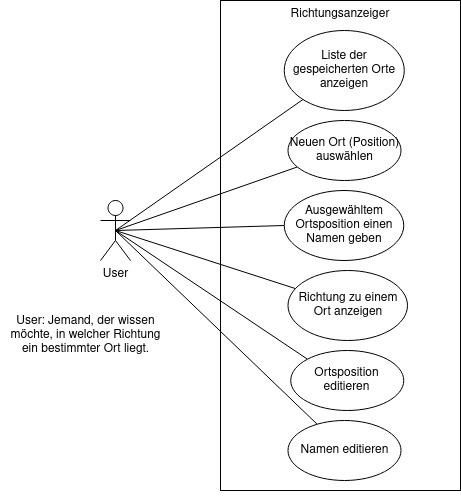
\includegraphics[width=10.0cm]{../UseCase.jpg}

\subsection{Nicht-funktionale Anforderungen}

\begin{itemize}
  \item Die Sprache der Benutzeroberfläche ist Deutsch.
  \item Persistente Daten werden mit SharedPreferences verwaltet.
  \item Zielplattform ist Android 8.1.
\end{itemize}

% \section{Testkonzept}
%
% \section{Aufbau des Systems}
%
% \section{Visualisierung des Gesamtsystems}

\end{document}
